% The original template (from Trevor) had a custom \appendix command,
% but I found it to break figure/table counters. I'm not sure how
% reliable my fix is, so I ended up reverting back to the standard
% latex version, and renaming the custom command to \myappendix.  You
% can try both and see how things work out:
% 1) Call \appendix once, and then make each appendix a \chapter
% 2) Call \myappendix once, and then make each appendix a \section.

\appendix
\chapter{Appendix Title}



\section{Detailed System Design of Perpendicular station}


We have developed one of the most sensitive Spin-torque ferromagnetic resonance perpendicular magnetic stations. Here we describe the detailed system designs.


\begin{figure*}[t]
  \centering
  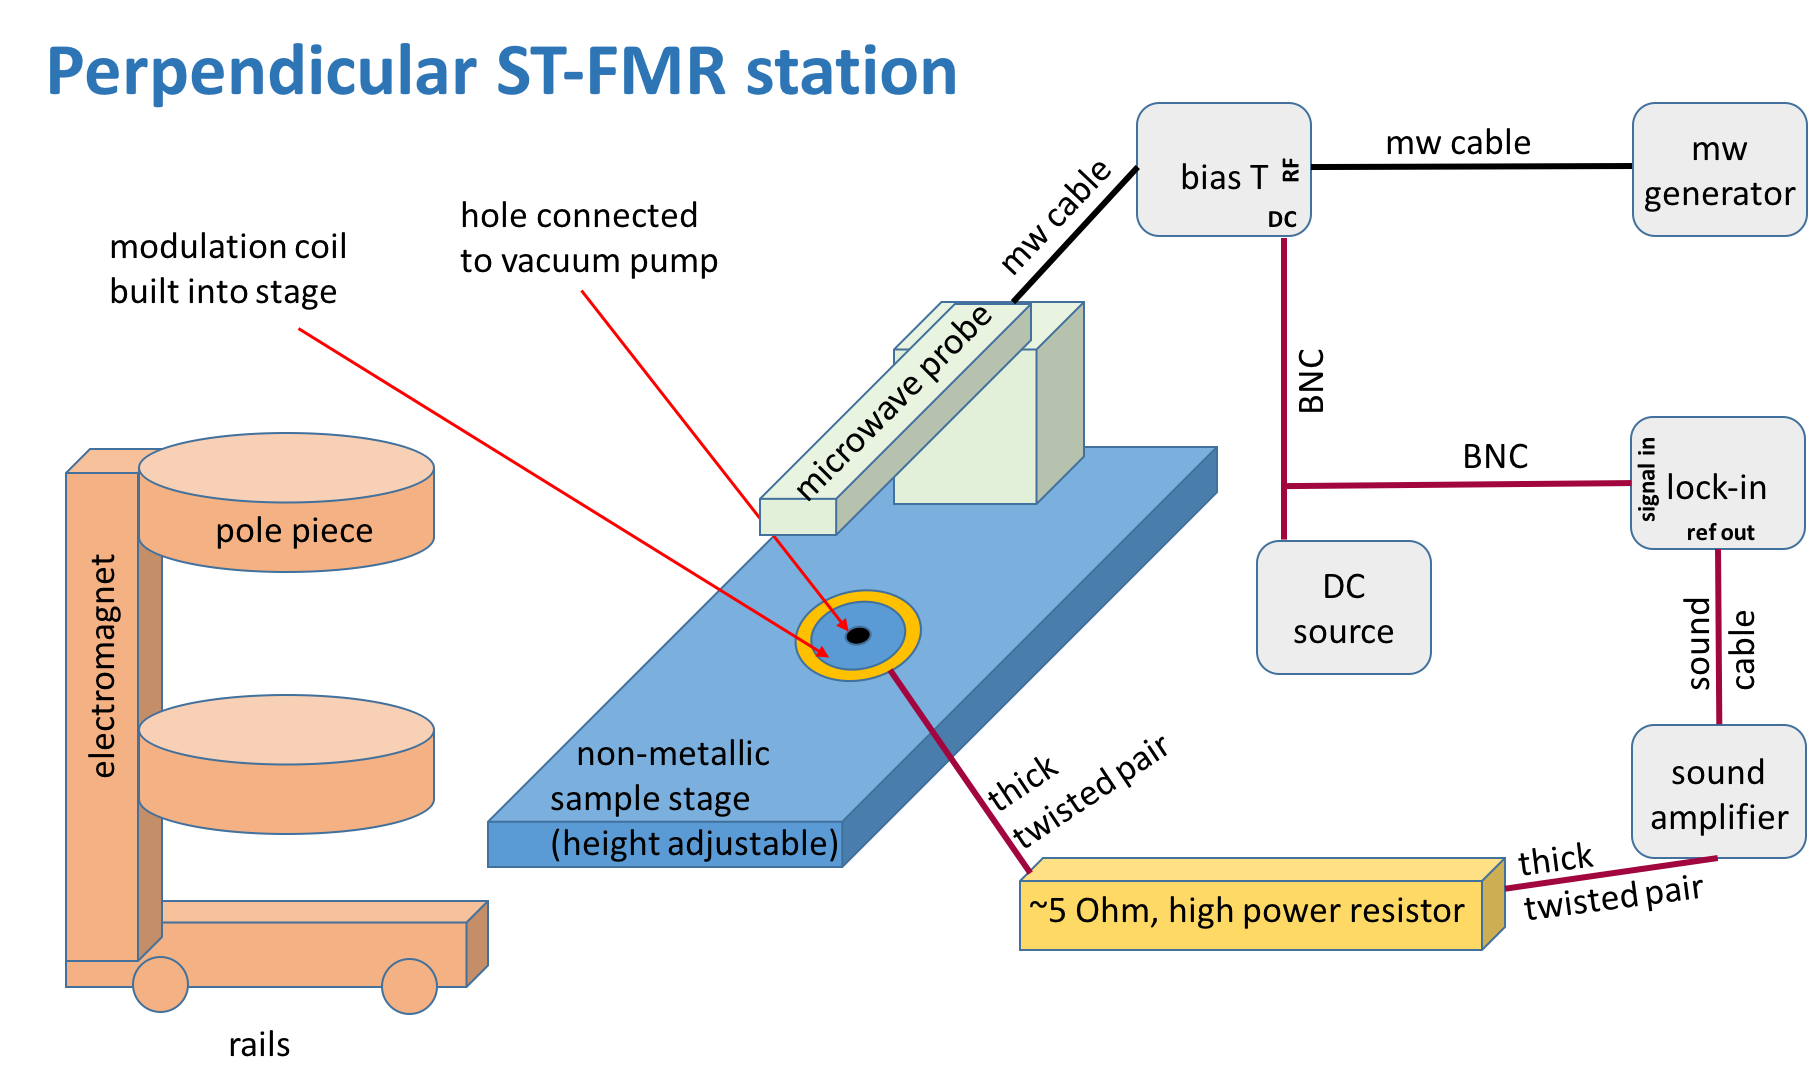
\includegraphics[width=1.0\textwidth]{fig/appendix/setup.png}
  \caption{Perpendicular ST-FMR station Setup}
  \label{fig:stationsetup}
\end{figure*}



First of all, here is all the equipments needed to build the out-of-plane magnetic probe station:

\begin{enumerate}
  \item GMW Dipole Electromagnet Model 3470
  \item Kepco bipolar operational power supply model Model 50-8M 
  \item Cascade RF probe : SG-120um
  \item Cascade RPP210-AI probe positioner (both the probe and the positioner are non-magnetic)
  \item Sentech Output 720p Cased Camera
  \item Navitar 12X Zoom Lens System
  \item AmScope LED-80M 80-LED Microscope Ring Light
\end{enumerate}

Fig.\ref{fig:stationsetup} sketches the design of the out-of-plane station.The magnet is fixed vertically on metal frame and the stage height is adjustable. At first, we can land the probe to make contact of the sample with the magnet moving away(shown in Fig.\ref{fig:operation1}. After making contact of the sample, first remove the camera (the setup could be improved by making a stationary camera). Then we can slide in the magnet so that the sample is located in the center of the magnet. It is important not to touch the probe and microwave cable when sliding the magnet. After moving the magnet we are ready to make ST-FMR measurement as showing in Fig.\ref{fig:operation2}.


\begin{figure}[!ht]
\centering
\subfigure{\label{fig:operation1}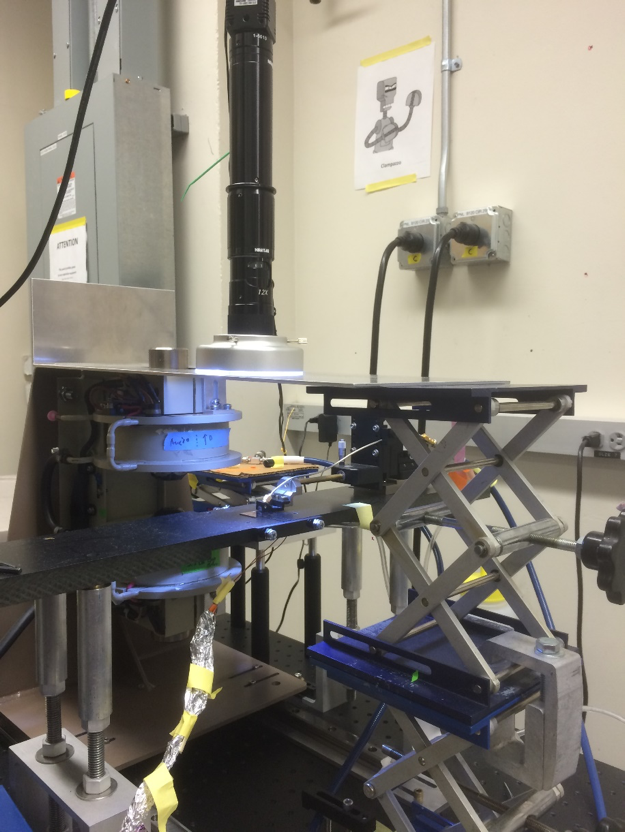
\includegraphics[width=75mm]{fig/appendix/1.png}}
\subfigure{\label{fig:operation2}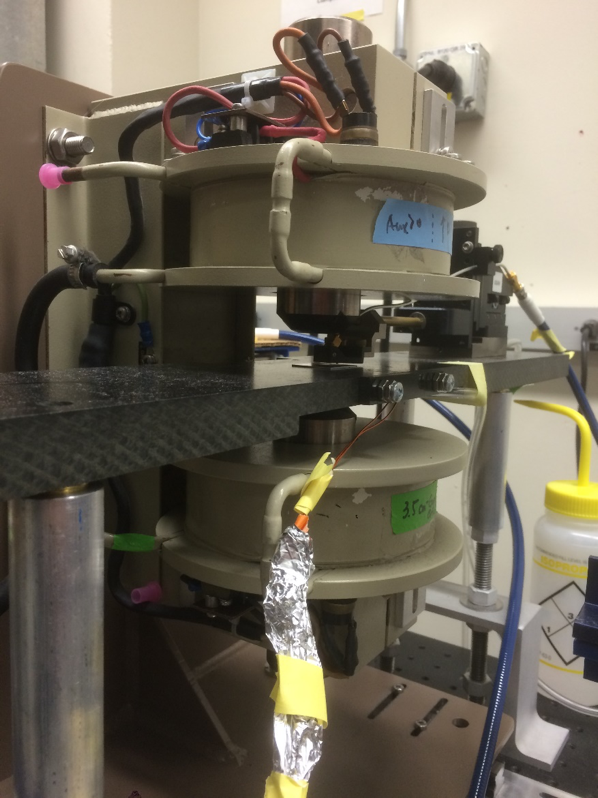
\includegraphics[width=75mm]{fig/appendix/2.png}}
\caption{Operation of Out-of-plane probe station}
\end{figure}


\begin{figure}[!ht]
\centering
\subfigure{\label{fig:operation3}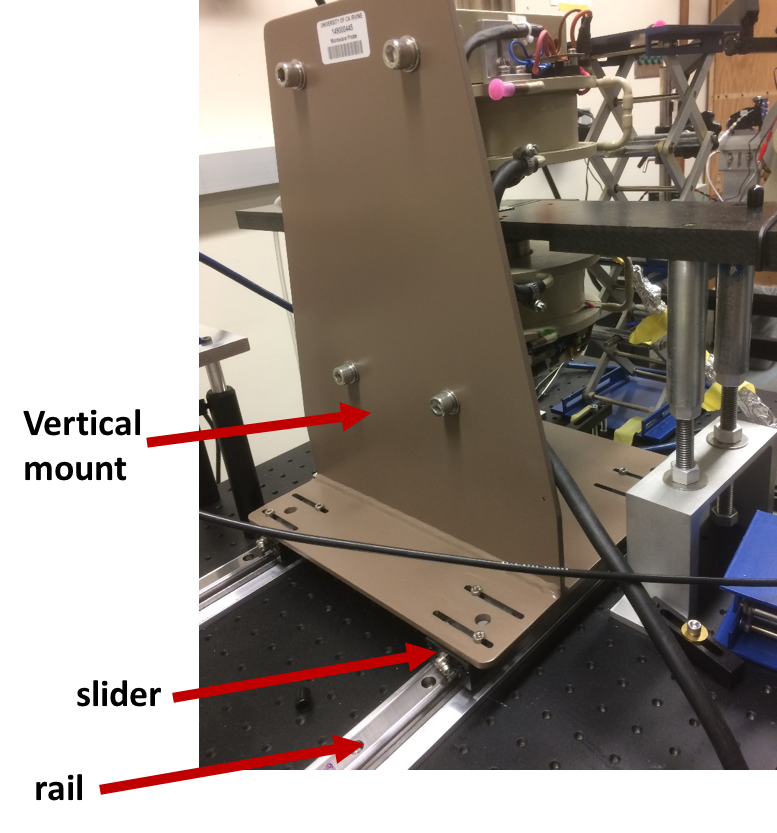
\includegraphics[width=75mm]{fig/appendix/3.png}}
\subfigure{\label{fig:operation4}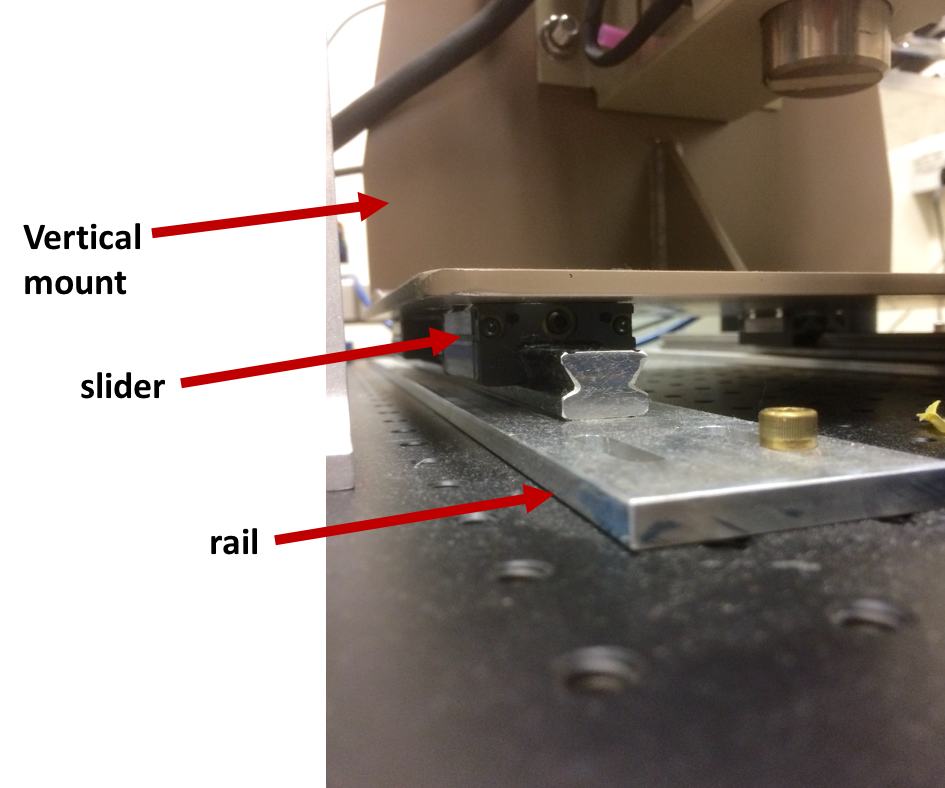
\includegraphics[width=75mm]{fig/appendix/4.png}}
\caption{(a) Side view of the magnet. (b) Bottom view of the magnet}
\end{figure}


Here is the list of equipments needed for making ST-FMR measurements up to 40 GHz.

\begin{enumerate}
  \item Signal recovery 7225 DSP lock-in Amplifier
  \item Hittite HMC-T2240 synthesized signal generator, 10 MHz to 40 GHz
  \item Clear Microwave Broadband Bias Tee BT50K40 50Khz-40GHz
  \item Keithley 2400 Source Meter (DC Source)
  \item Microwave cable : Teledyne Accutest R95-0004-072 (72 inch 1GHz- 40GHz)
  \item Pomona BNC cables

\end{enumerate}

When connecting the microwave cables, there are two small things worth notice. Firstly, all the connectors should be cleaned regularly. Secondly, the microwave cables should be supported to release all the possible tensions.

\begin{figure*}[t]
\centering
\subfigure{\label{fig:operation5}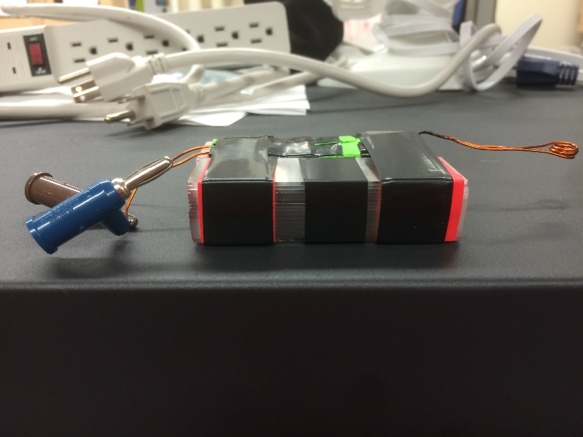
\includegraphics[width=75mm]{fig/appendix/5.png}}
\subfigure{\label{fig:operation6}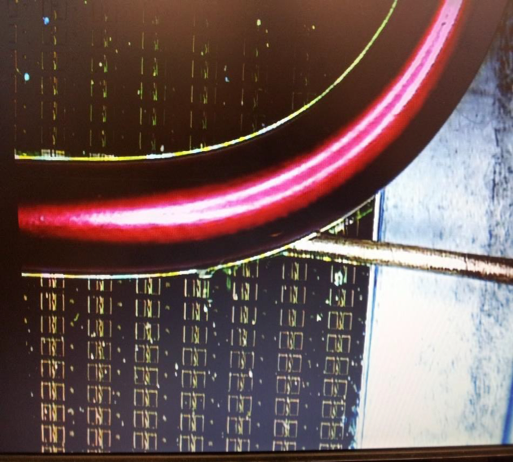
\includegraphics[width=75mm]{fig/appendix/6.png}}
\caption{(a) Coil for out-of-plane modulation (b) Wire for in-plane modulation}
\end{figure*}

The last pieces of equipments needed is the field modulation setup. Here is the list:

\begin{enumerate}
  \item Behringer EUROPOWER Professional 4,000-Watt Stereo Power Amplifier 
  \item TE CONNECTIVITY / CGS CJT10004R7JJ  Through Hole Wire wound Resistor, 4.7 Ohm
  \item High quality cable connecting from lock-in to the input of the sound amplifier : Monster Performer 500 - 10' Speaker Cable
  \item BK Precision 2831E  Ammeter to control the current through the copper wire  
\end{enumerate}
  
 When making the field-modulation coil, it is better to use any low resistance copper wire for magnetic field modulation coil. For out-of-plane field modulations, we use an external coil above the sample as shown in Fig.\ref{fig:operation5}. In-plane field modulation can be achieved by simply placing straight wire above the sample as shown in Fig.\ref{fig:operation6}. In our current design, we embed the coil into the plastic base right under the sample. It is important to ensure that the wire is not in contact with the sample or any other parts of the microwave setup. 


\begin{figure*}[h]
\centering
\subfigure{\label{fig:operation7}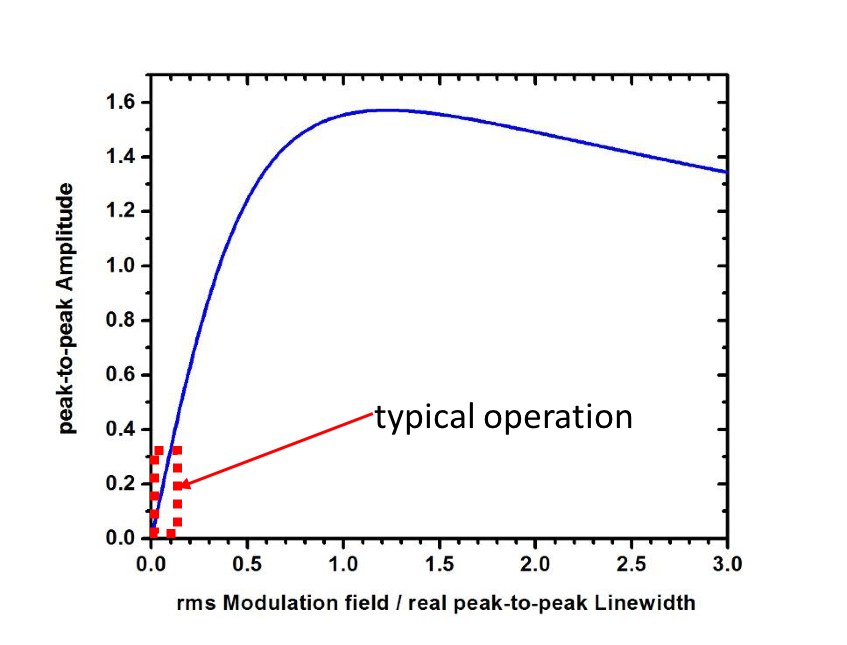
\includegraphics[width=80mm]{fig/appendix/7.png}}
\subfigure{\label{fig:operation8}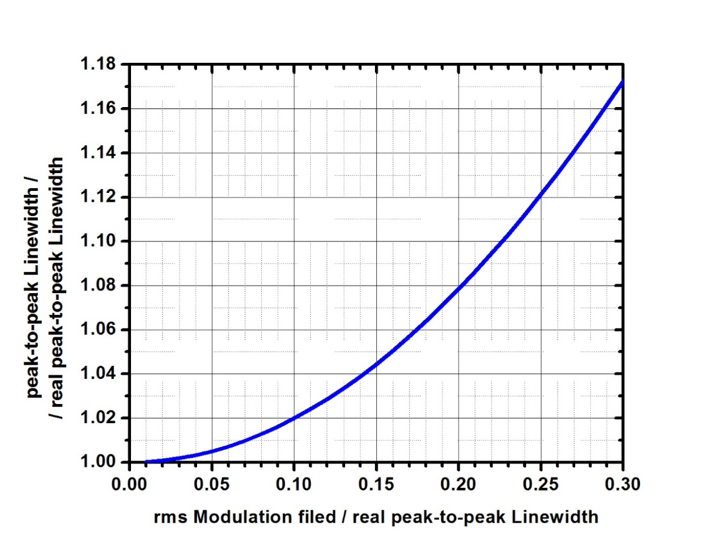
\includegraphics[width=80mm]{fig/appendix/8.png}}
\caption{(a) Peak-to-peak amplitude versus rms modulation field over real peak-to-peak linewidth. (b) peak-to-peak linewidth over real peak-to-peak linewidth versus rms modulation field over real peak-to-peak linewidth.}
\end{figure*}

In the experiment, two parameters need to be determined for the field modulation: the amplitude of modulation field and the frequency of the modulation ac field. Typically Increasing the modulation field increases the signal amplitude, but not infinitely as shown in Fig.\ref{fig:operation7}. If you are over-modulating, the signal becomes distorted and the linewidth broadens as shown in Fig.\ref{fig:operation8}. In our current setup, the input ac current is about 3.6 A to achieve the modulation field around a few oersted field, which is enough to have decent signal-to-noise ratio without distorting the spectrum.





\clearpage




%%% Local Variables: ***
%%% mode: latex ***
%%% TeX-master: "thesis.tex" ***
%%% End: ***
